\documentclass[border=12pt]{standalone}
\usepackage{tikz}
\usepackage{amsmath}
\usetikzlibrary{positioning,arrows.meta,fit,backgrounds,calc}
\begin{document}
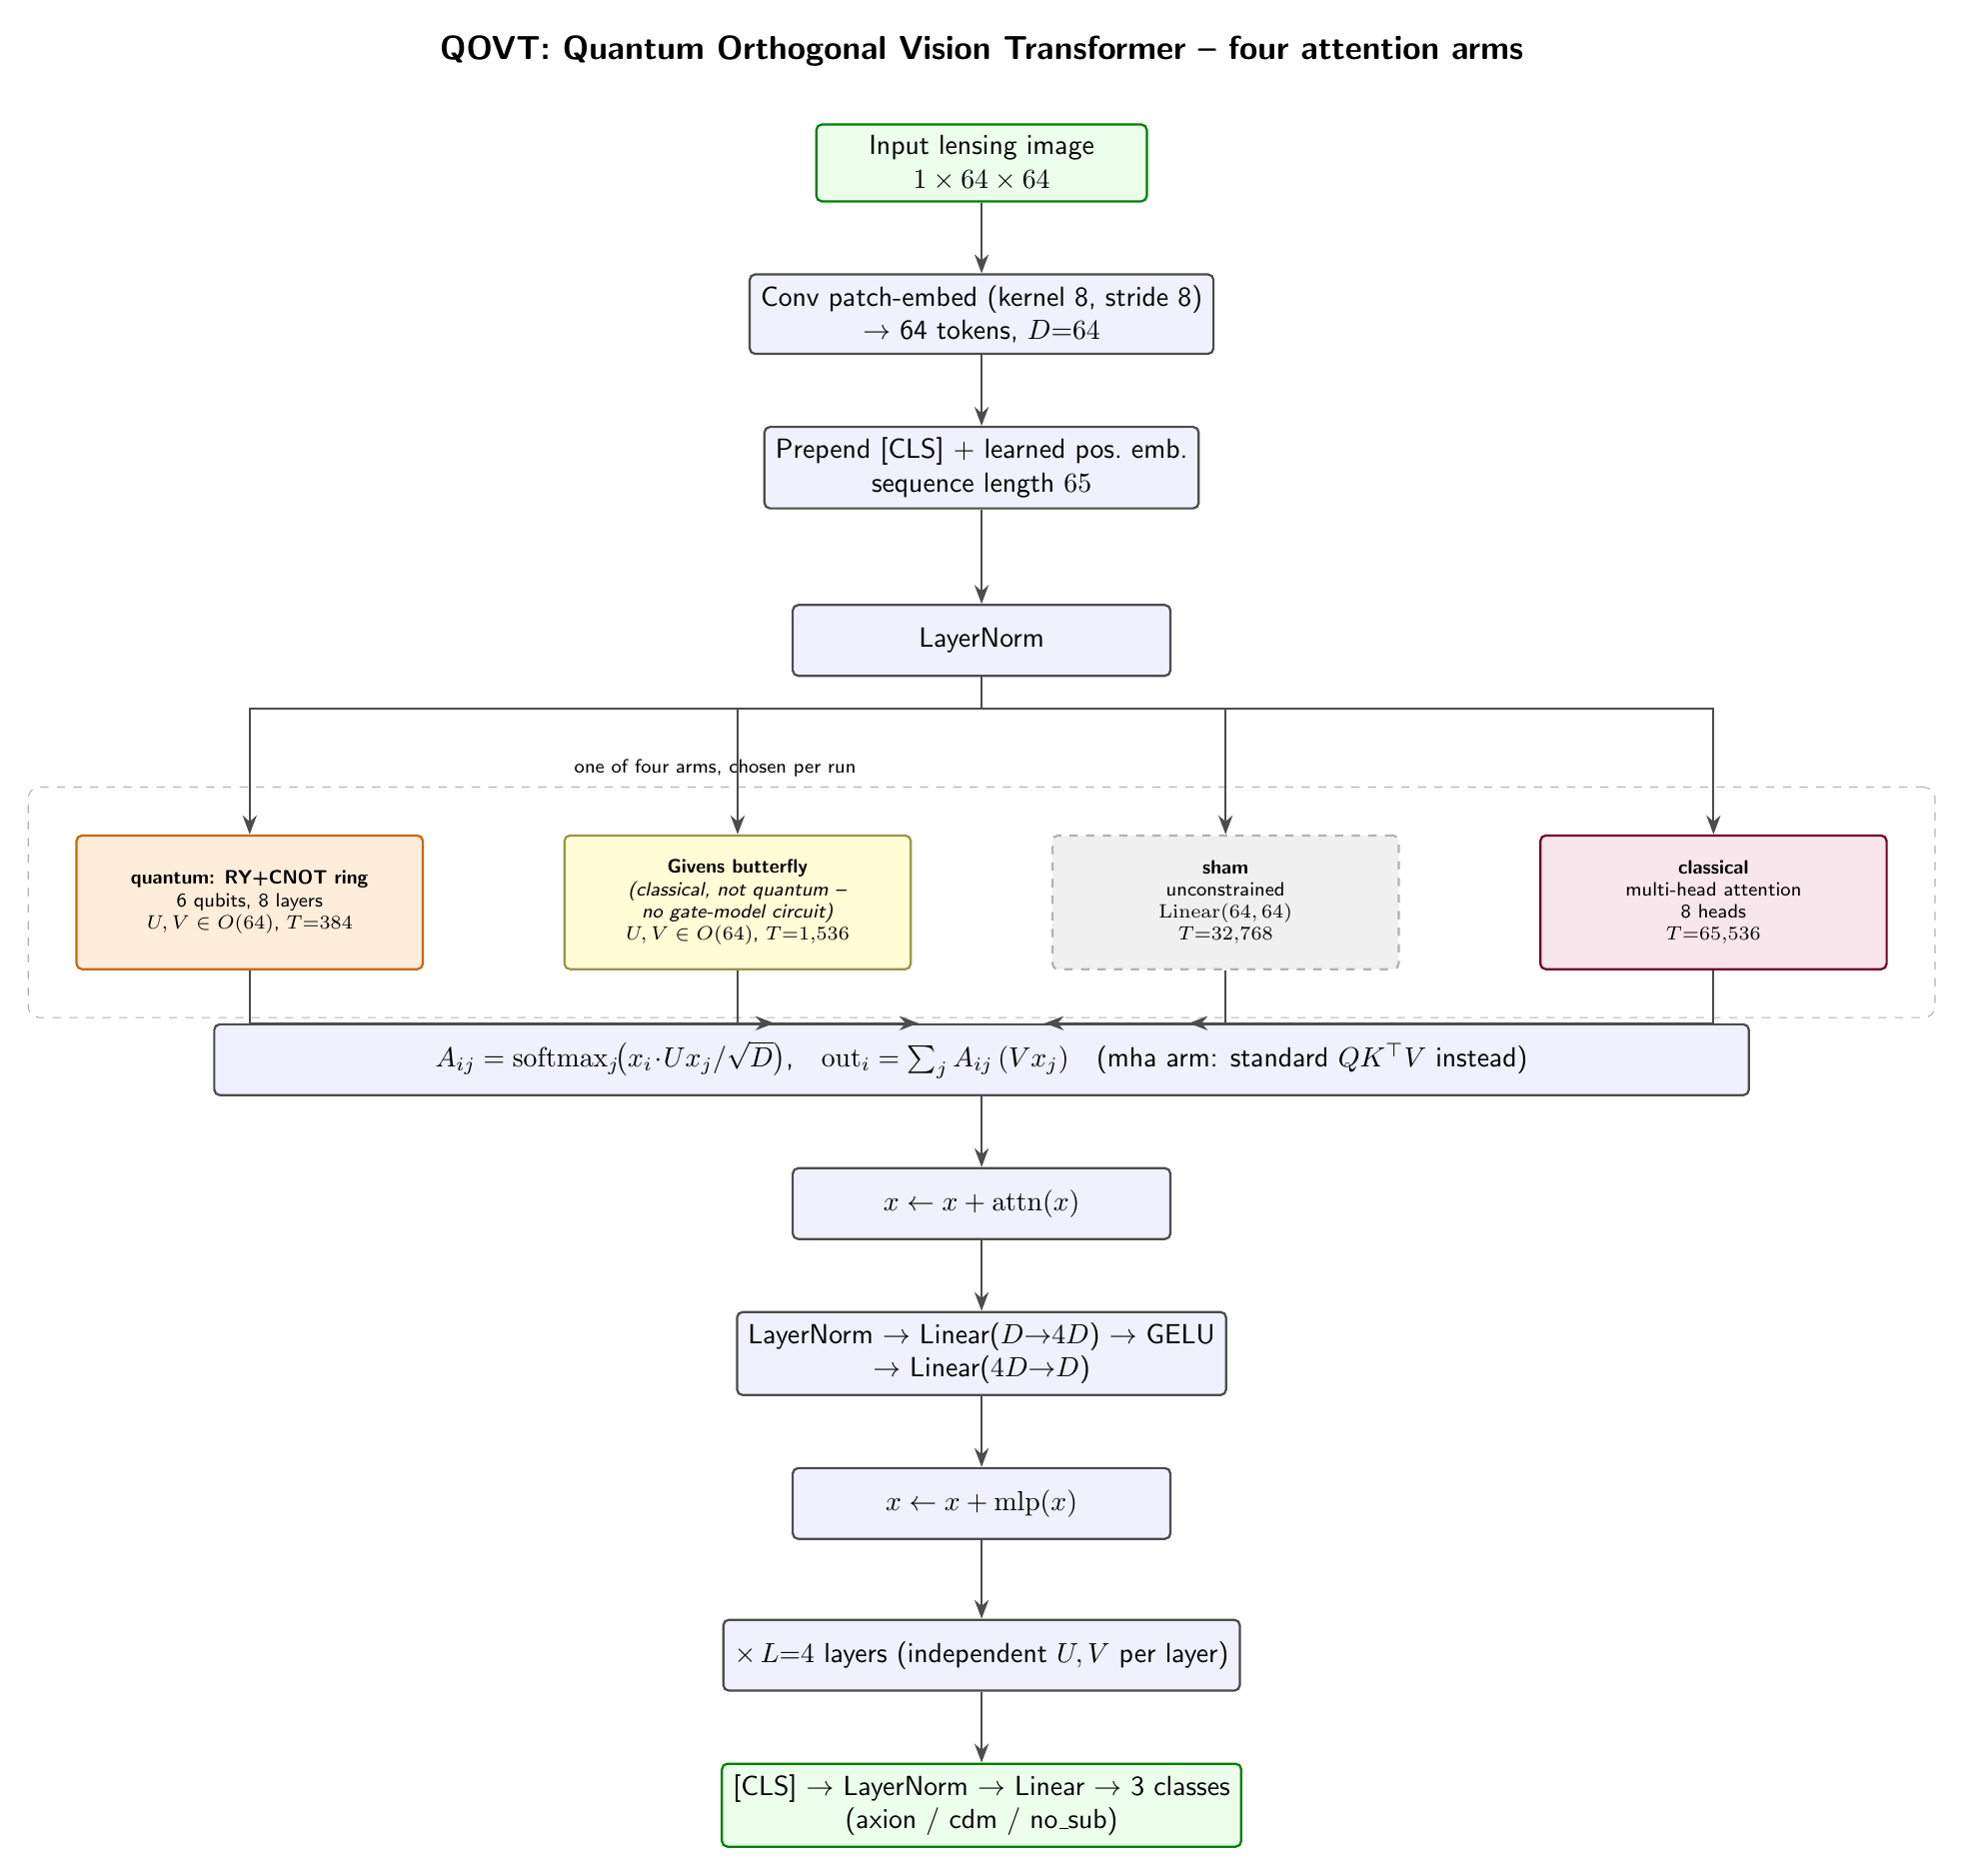
\begin{tikzpicture}[
  font=\sffamily,
  node distance=9mm,
  box/.style={rectangle,rounded corners=2pt,draw=black!70,thick,fill=blue!6,
              minimum height=9mm,minimum width=42mm,align=center,inner sep=4pt},
  qbox/.style={box,fill=orange!14,draw=orange!80!black,minimum width=44mm,
               minimum height=17mm,font=\sffamily\scriptsize},
  gvbox/.style={qbox,fill=yellow!16,draw=yellow!55!black},
  shbox/.style={qbox,fill=gray!12,draw=gray!60,dashed},
  clbox/.style={qbox,fill=purple!10,draw=purple!60!black},
  io/.style={box,fill=green!8,draw=green!50!black},
  arr/.style={-{Stealth[length=2.4mm]},thick,black!70},
]

% ---- backbone (shared across all 4 arms) ----
\node[io] (img) {Input lensing image\\$1\times64\times64$};
\node[box,below=of img] (patch) {Conv patch-embed (kernel 8, stride 8)\\$\to$ 64 tokens, $D{=}64$};
\node[box,below=of patch] (cls) {Prepend [CLS] + learned pos.\ emb.\\sequence length $65$};

% ---- one QO-attention layer, expanded to show the 4 arms (repeated $L{=}4\times$) ----
\node[box,below=12mm of cls,minimum width=48mm] (norm) {LayerNorm};

\node[qbox,below=20mm of norm,xshift=-93mm] (ry)
  {\textbf{quantum: RY+CNOT ring}\\6 qubits, 8 layers\\$U,V\in O(64)$, $T{=}384$};
\node[gvbox,below=20mm of norm,xshift=-31mm] (bf)
  {\textbf{Givens butterfly}\\\textit{(classical, not quantum --}\\\textit{no gate-model circuit)}\\$U,V\in O(64)$, $T{=}1{,}536$};
\node[shbox,below=20mm of norm,xshift=31mm] (sham)
  {\textbf{sham}\\unconstrained\\$\mathrm{Linear}(64,64)$\\$T{=}32{,}768$};
\node[clbox,below=20mm of norm,xshift=93mm] (mha)
  {\textbf{classical}\\multi-head attention\\8 heads\\$T{=}65{,}536$};

\node[box,below=44mm of norm,minimum width=195mm]
  (attn) {$A_{ij}=\mathrm{softmax}_j\!\big(x_i\!\cdot\!Ux_j/\sqrt{D}\big)$,\quad
          $\mathrm{out}_i=\sum_j A_{ij}\,(Vx_j)$\quad(mha arm: standard $QK^\top V$ instead)};

\node[box,below=of attn,minimum width=48mm] (res1) {$x \gets x + \mathrm{attn}(x)$};
\node[box,below=of res1,minimum width=48mm] (mlp)
  {LayerNorm $\to$ Linear($D{\to}4D$) $\to$ GELU\\$\to$ Linear($4D{\to}D$)};
\node[box,below=of mlp,minimum width=48mm] (res2) {$x \gets x + \mathrm{mlp}(x)$};

\node[box,below=10mm of res2,minimum width=64mm] (repeat)
  {$\times\,L{=}4$ layers (independent $U,V$ per layer)};

\node[io,below=of repeat] (out) {[CLS] $\to$ LayerNorm $\to$ Linear $\to$ 3 classes\\(axion / cdm / no\_sub)};

\draw[arr] (img)--(patch);
\draw[arr] (patch)--(cls);
\draw[arr] (cls)--(norm);
\draw[arr] (norm.south) -- ++(0,-4mm) -| (ry.north);
\draw[arr] (norm.south) -- ++(0,-4mm) -| (bf.north);
\draw[arr] (norm.south) -- ++(0,-4mm) -| (sham.north);
\draw[arr] (norm.south) -- ++(0,-4mm) -| (mha.north);
\draw[arr] (ry.south)   |- (attn.170);
\draw[arr] (bf.south)   |- (attn.150);
\draw[arr] (sham.south) |- (attn.30);
\draw[arr] (mha.south)  |- (attn.10);
\draw[arr] (attn)--(res1);
\draw[arr] (res1)--(mlp);
\draw[arr] (mlp)--(res2);
\draw[arr] (res2)--(repeat);
\draw[arr] (repeat)--(out);

\begin{scope}[on background layer]
\node[fit=(ry)(bf)(sham)(mha),draw=black!30,dashed,rounded corners=4pt,
      inner sep=6mm,label={[font=\sffamily\scriptsize]above left:one of four arms, chosen per run}] {};
\end{scope}

\node[font=\sffamily\large\bfseries,above=6mm of img]
  {QOVT: Quantum Orthogonal Vision Transformer -- four attention arms};
\end{tikzpicture}
\end{document}
